 
%\documentclass[review]{elsarticle}
\documentclass[final,twocolumn]{elsarticle}
%\documentclass[final,5p,times,twocolumn]{elsarticle}

\usepackage{project}

%! Author = sbbfti
%! Date = 10/06/2020

\newacronym{ADF}{ADF test}{Augmented Dickey-Fuller test}
\newacronym{KPSS}{KPSS test}{Kwiatkowski-Phillips-Schmidt-Shin test}
\newacronym{ACF}{ACF}{AutoCorrelation function}
\newacronym{PACF}{PACF}{Partial AutoCorrelation function}


\newacronym{ti}{$T_{i}$}{indoor air temperature, $^{\circ}$C}


\begin{document}

    \begin{frontmatter}

\title{Footprint Recognition}


%% Group authors per affiliation:
\author{Saeed Kazemi\fnref{myfootnote}}
\address{University of New Brunswick}
\fntext[myfootnote]{Saeed.Kazemi@unb.ca.}

%% or include affiliations in footnotes:
\ead[url]{https://github.com/SKazemii/EE6563}

\begin{abstract}
Given present-day security concerns, many buildings have implemented robust authentication techniques. Aside from authentication to enter a building, applications such as border and airport security also administer identification. Because of these needs, many cities and companies provide technologies like CCTV or fingerprinting for authentication and verification. But each system has its own issue. For example, due to the Covid-19 pandemic, most people wear a mask and avoid touching unnecessary surfaces. This aids to disguise people and reduces the hygiene of fingerprint biometrics respectively. In this research, we focus on which classifier has better results on barefoot footprints and which features have the important effect on the classifier.
\end{abstract}

\begin{keyword}
Footprint\sep Time series\sep pressure sensor
\end{keyword}

\end{frontmatter}

    \section{Introduction}

Contemporary security identification has led to a plethora of biometric-based authentication systems. From palm readers at testing centers to facial recognition on smartphones, many systems are now used to regularly verify identities. These inherence-based systems are attractive in comparison to knowledge or possession-based methods of authentication because biometrics are highly unique, unforgettable, and far more difficult to steal than a password or swipe card.

Although biometric identification appears sophisticated when compared to something like physical keys, it does not come without its own share of caveats. For example, due to the ongoing Covid19 pandemic, many people wear masks when outside of their house, challenging most facial recognition systems. Additionally, biometrics that rely on touch, such as fingerprinting, raise safety concerns, as the scanner may become a vector for virus transmission. Despite these setbacks, given their merits and widespread deployment, biometric identification systems are unlikely to disappear.

One behavioral biometric that has gained recent success and is worth further consideration given current constraints is gait recognition. Usage of gait recognition has grown in the security industry in recent decades due to advances in deep learning. Singh et al. \cite{Singh2019APerspectives} categorized gait recognition into two main categories, vision-based and sensor-based. In vision-based approaches, cameras capture data of a person walking for the purpose of gait recognition. Sensor-based gait recognition is performed using either wearable sensors which produce kinematic data, or floor sensors which produce kinetic data \cite{Connor2018BiometricFeatures}.


\section{Datasets}
This project uses two different datasets, UoM-Gait-Dataset and Stepscan. The UoM-Gait-Dataset was obtained from iMAGiMAT sensor \cite{Cantoral-Ceballos2015IntelligentEnvironments} (an optical floor sensor). This sensor contains about 160 distributed \gls{pof} that indicate the foot pressure signals over time. Some studies like \cite{Costilla-Reyes2020DeepHealthcare} use this dataset to construct an image for their research.

The second dataset that was used for this project is called the Stepscan dataset \cite{Connor2015ComparingBiometrics}. This dataset was obtained from high-resolution floor tiles that has recently introduced by Stepscan Technologies Inc.

Figure \ref{fig:Stepscan_dataset} indicates three frames from this dataset. This dataset consists of a spatial-temporal tensor, X, with dimensions $S \times T \times H \times W$ where S represents the number of samples. T is the number of temporal observations or video frames, H and W are the dimension of the image in pixels. Moreover, both datasets include different walking speeds information. 

This project aims to find some temporal features from the datasets to construct a classifier for verification duty. The nature of data in the first dataset is time series, whereas Stepscan is an video base dataset. There are several methods for converting a tensor (like video) to the 2D time-series data. 

Chen et al. in \cite{Chen2006GaitModel} used contour width for defining a one-dimensional signal. They utilized some morphological operations on the background-subtracted silhouette image to extract the outer contour. Afterwards, according to the contour width of each image row, a one-dimensional signal was generated.

Another method could be that the pixel values in each frame are plot over time. Therefore, the $H * W$ time-series will produce for each sample.

In the final method, some spatial features are extracted from each frame (e.g. centroid and maximum pressure in each image). Afterwards, we track these values over time (next frames). As a result, 3D videos with size $T \times H \times W$ convert to the four 2D time-series data. Costilla-Reyes et al. utilized this method to combine the output of 160 distributed \gls{pof} \cite{Costilla-Reyes2018DeepSensors}.

In this research, the last mentioned method was applied to produce time-series data. Figure \ref{fig:extracted_features} indicates the time series extracted from the Stepscan dataset. The spatial features extracted in each frame were maximum pressure (figure \ref{fig:extracted_features_max}), the center of pressure (COP) (figures \ref{fig:extracted_features_yCe} and \ref{fig:extracted_features_xCe}), and the average pressure (figure \ref{fig:extracted_features_sum}). 





%As the figure \ref{fig:Stepscan_dataset} shows the data is a image not a time series data. Therefore, we need to convert our data to a time series. 

\begin{figure}
    \centering
    \begin{minipage}[b]{.5\textwidth}
        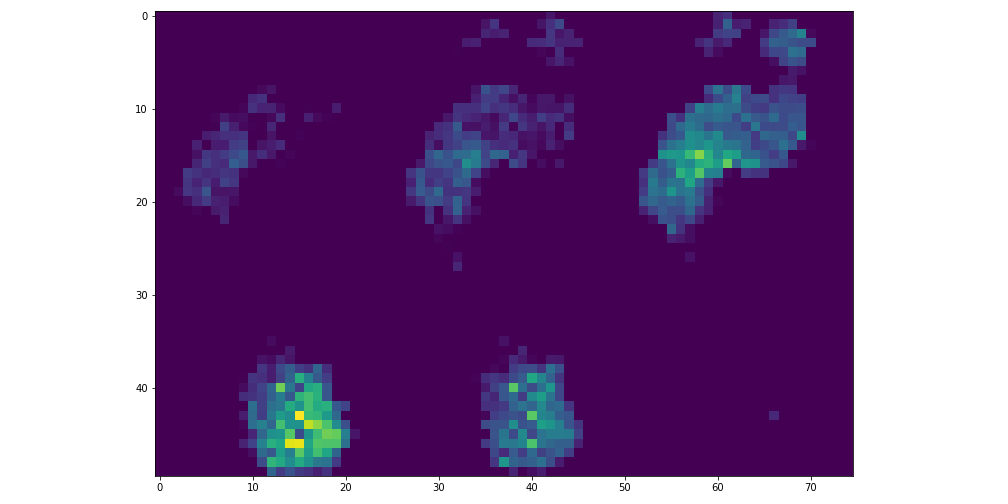
\includegraphics[width=\textwidth]{figures/project/frame1.png}
    \end{minipage}
    \caption{Different frames of footprint video in Stepscan dataset.}
    \label{fig:Stepscan_dataset}
\end{figure}


\begin{figure}
     \centering
     \begin{subfigure}[b]{0.5\textwidth}
         \centering
         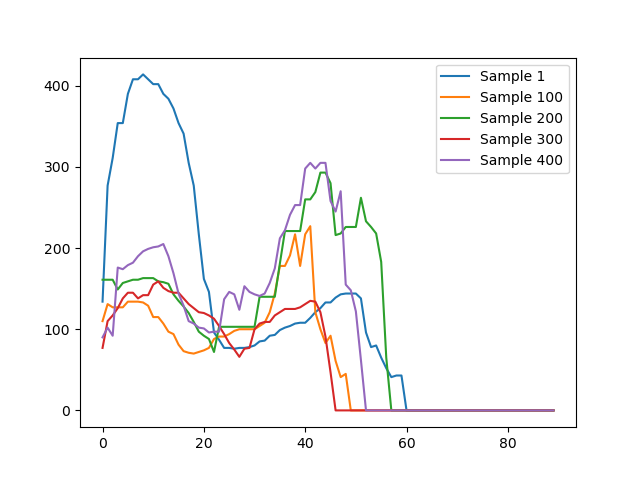
\includegraphics[width=\textwidth]{figures/project/df_max.png}
         \caption{The maximum pressure in each frame}
         \label{fig:extracted_features_max}
     \end{subfigure}
     \hfill
     \begin{subfigure}[b]{0.5\textwidth}
         \centering
         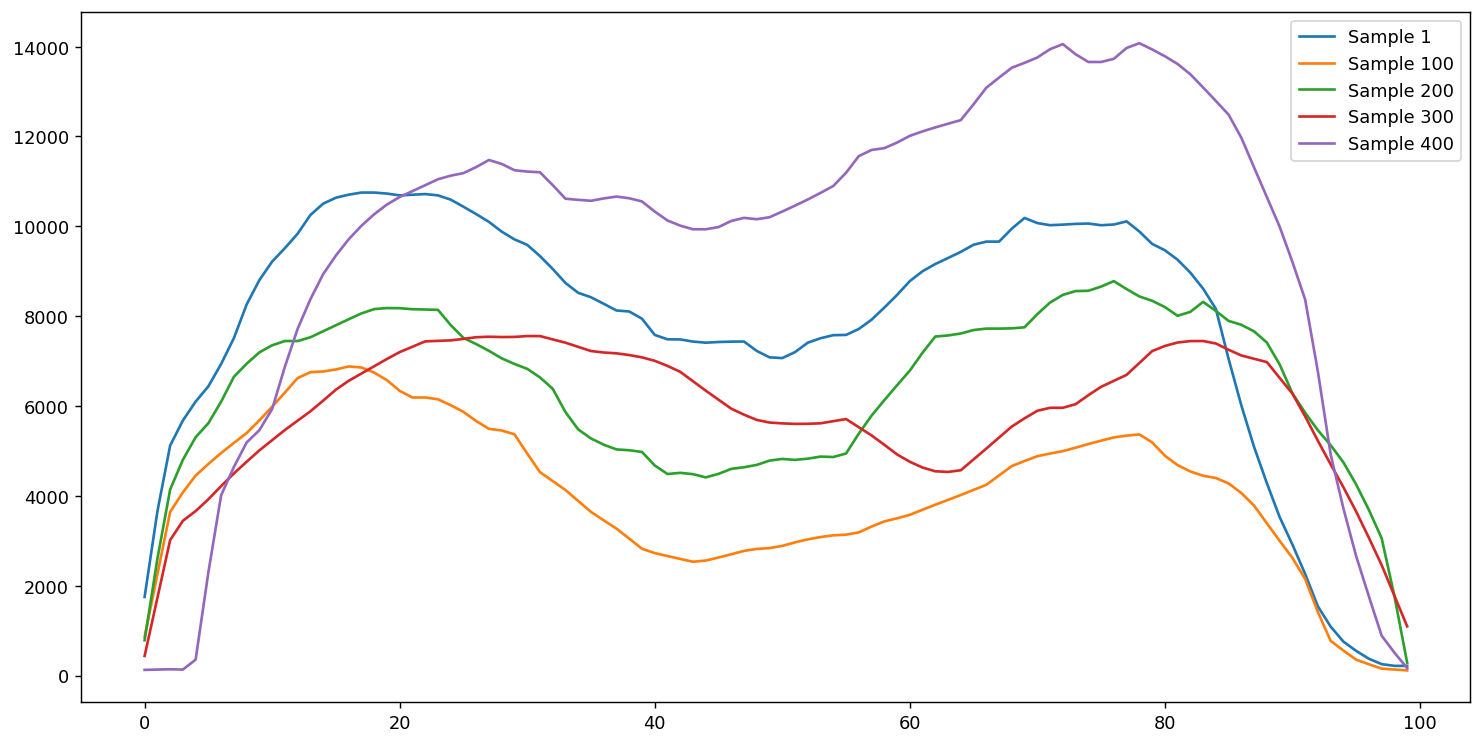
\includegraphics[width=\textwidth]{figures/project/df_sum.png}
         \caption{The average pressure in each frame}
         \label{fig:extracted_features_sum}
     \end{subfigure}
     \vfill
     \begin{subfigure}[b]{0.5\textwidth}
         \centering
         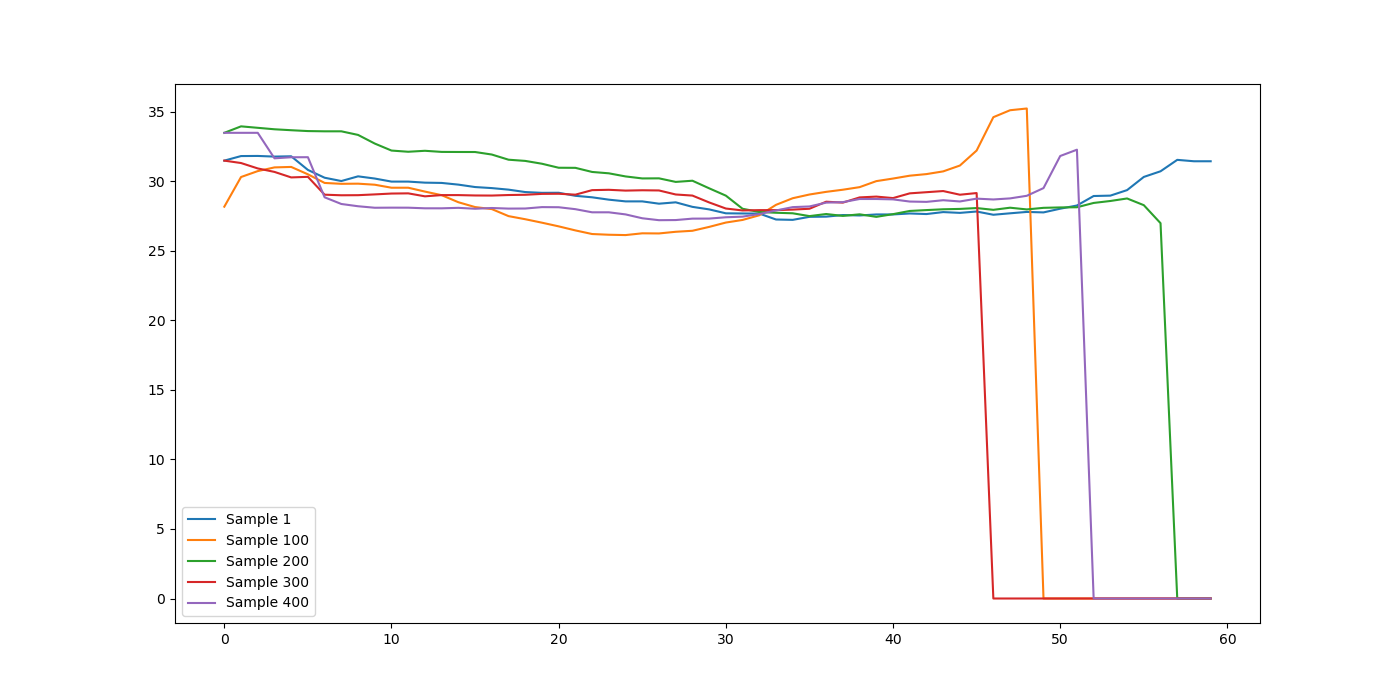
\includegraphics[width=\textwidth]{figures/project/df_xCe.png}
         \caption{The x position in the center of pressure (COP) in each frame}
         \label{fig:extracted_features_xCe}
     \end{subfigure}
     \hfill
     \begin{subfigure}[b]{0.5\textwidth}
         \centering
         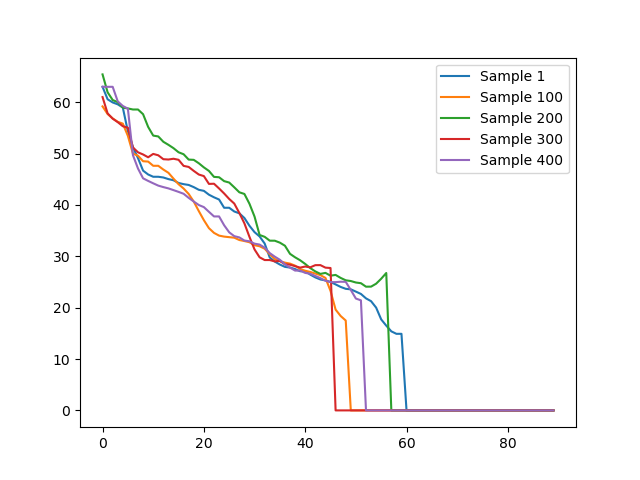
\includegraphics[width=\textwidth]{manuscript/src/figures/project/df_yCe.png}
         \caption{The y position in the center of pressure (COP) in each frame}
         \label{fig:extracted_features_yCe}
     \end{subfigure} 
        \caption{The time series extracted from the Stepscan dataset based on four spatial features. The horizontal axis indicates the frame number.}
        \label{fig:extracted_features}
\end{figure}






    \section{Methodology}

\subsection{The subsection also appears in the bookmarks}

    \section{Constraints}
The constraints in this project could fall into two groups. The first constraint is related to the limitation on laboratory conditions \cite{Connor2018BiometricFeatures}. In real-world circumstances, many situations such as walking speed, clothing, footwear, and load carriage could affect our results, whereas our datasets could cover some of these real-world conditions. For example, except for the walking speed and footwear, both datasets do not have useful information for other real-world situations. Consequently, our results are optimistically biased. Table \ref{tab:1_vul} indicates some inhibiting factors. 

Another significant limitation in the Stepscan dataset is the lack of relative footprint location. The dataset included only aligned and segmented footprint images. The location of samples concerning each other is unknown. This information could play a significant role in predicting the location of future footsteps. 

 

\section{Proposed Work}

There are two modes for footprint recognition or generally in the biometric system: verification or identification mode \cite{Jain2004AnRecognition}. In verification mode, the biometric system use for accessing buildings or data. In other words, the system compares the claimed person with its dataset to determine whether or not the claim is valid. These systems consume less processing power and time consumption \cite{Jain2004AnRecognition}. 



This project will focus on verification. Since each participant has multiple samples in our dataset, we hope to find some temporal features. These features help us to construct a classifier which can discriminate between our dataset’s various participants. Since both datasets contain various walking speeds, it would be a good idea to find a classifier based on the participants' speeds.

In recent years, improving the computational process of computers and other benefits of \gls{dnn} causes many researchers (like \cite{IsmailFawaz2019DeepReview} and \cite{Costilla-Reyes2018DeepSensors}) to move towards \gls{dnn} for the classification of time series data. Therefore, these algorithms will review in this project. 



Having spatial features along with temporal information give us a freedom to select and combine many classifiers in the pipeline to increase our accuracy. We also plan to use some techniques learned in time-series analysis course hopefully elicit some useful features for future works.
 
Furthermore, this research will employ two available datasets (UoM-Gait-Dataset and Stepscan), and will be implemented in python. The source codes are available on the GitHub repository \cite{SKazemii/EE6563}. 

\begin{center}
	\begin{table}[!t]
	\caption{Some inhibiting factors in gait recognition.}
	\label{tab:1_vul}
	\hspace{3em}
%	\setlength\extrarowheight{-2pt}
	\begin{tabular}{rl}
\toprule
    &  Inhibit Factors \\
\midrule
  1 & Footwear               \\
  2 & clothing               \\
  3 & Injury                 \\
  4 & Muscle development     \\
  5 & Fatigue                \\
  6 & Age                    \\
  7 & Load carriage          \\
  8 & Walking speed          \\
  
\bottomrule
\end{tabular}


	\end{table}
\end{center}
%    \newpage
    \section{CNN}



\paragraph{Functionality} The Elsevier article class is based on the standard article class and supports almost all of the functionality of that class. In addition, it features commands and options to format the
\begin{itemize}%\begin{enumerate}[(1)]
\item document style
\item baselineskip
\end{itemize}



\begin{figure}
    \centering
    \begin{minipage}[b]{.5\textwidth}
        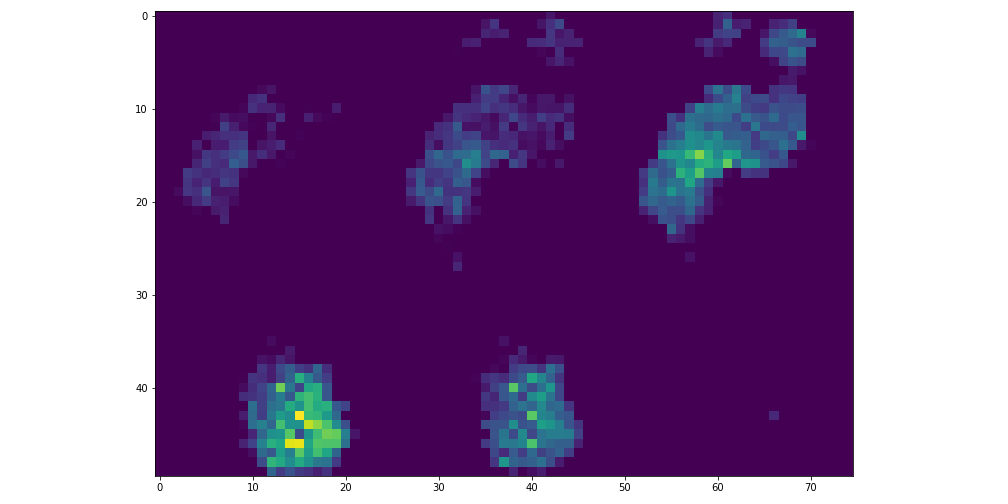
\includegraphics[width=\textwidth]{figures/project/frame1.png}
    \end{minipage}
    \caption{sample image.}
    \label{fig:Stepscan_dataset}
\end{figure}


Here are two sample references: \cite{SKazemii/EE6563}.
    
\section*{\#TODO:}
\begin{enumerate}[(1)]

\item You want to focus on temporal information, and how it will help.\\
\item add more to lead the reader into the next section. The project has not been "introduced".\\
\item Aren't they both time-series?  Are you just referring to the method that they are stored?   An array of images over time (video) is still a time series.\\ 
\item You should show them as separate frames; how can you show the temporal aspects better?\\
\item But these are just spatial features plotted over time? What are the proposed temporal features? \\
\item Are you only thinking about within cycle information?  What about inter-stride information?  (for example, inter-stride variability is a well known gait feature).\\
\item Have you explored relationships between pixels/features over time?
\item With what features? Costilla-Reyes et al. [17] extracted five features
\item Does Costilla-Reye's work deserve a bit more discussion?  Is that the current state-of-the-art?
\item This seems like it doesn't fit here.  Is this specific to gait?  Explain  
\item Are you sure?!  I believe that each frame has the [x,y] position of the center of the box.  We will need to get an answer for this soon as it changes what you can do.(inter-stride)
\item Focus on what is important; where is the temporal information going to come from?  Time series of spatial information?  Temporal features?  Temporal algorithms applied to spatial features?  Are the features only within stride, or are your features going to be inter-stride?
\item Is this the main benefit? (No)
\item Why does the fact that there are multiple samples mean you want to find temporal features (the first part of the sentence doesn't "cause" the second).
\item What do you mean "find one based on speed"?  Do you mean a different one depending on which speed?  I think you (should) mean designing a system that works for all speeds. 
\item This is still to "general" for a proposal.  It doesn't give me a good idea of what you are hoping to do.
\end{enumerate}    
    
%\nolinenumbers
\bibliography{references}
 



\onecolumn
\appendix
\section{List of features}
The list of features from different categories used in this project (Table \ref{tab:Features_list}):

{%\small
%\tablinesep=2ex\tabcolsep=10pt

\hspace{-6cm}
\begin{tabularx}{\linewidth}{@{}rlccc@{}}
\caption{list of features} \\
\label{tab:Features_list}\\
\toprule
  \#  &  Features Name & {Categories Name } & \# features & description\\
\midrule
\endfirsthead
\toprule
  \#  &  Features Name & {Categories Name } & \# features & description\\
\midrule
\endhead
\midrule
\multicolumn{4}{r}{\footnotesize( To be continued)}
\endfoot
\bottomrule
\endlastfoot

%  1 & ECDF              & Statistical  & A\\
%  2 & ECDF Percentile      & Statistical  & A         \\
%  3 & ECDF Percentile Count & Statistical  & A\\
  1 & Histogram    & Statistical  & 10 & 10-bin Histogram \\
%  5 & Interquartile range               & Statistical  & A \\
%  6 & Kurtosis                   & Statistical  & A \\
  2 & Max         & Statistical  & 1 & max(s)\\
  3 & Mean         & Statistical   & 1 & mean(s)\\
  4 & Mean absolute deviation         & Statistical   & 1 & ${\Sigma_{i=1}^{N} |S_i^2 - mean(s)|}/{N}$\\
  5 & Median         & Statistical   & 1 & median(s)\\
  6 & Median abs deviation         & Statistical   & 1 & $median(|s - median(s)|)$\\
  7 & Min         & Statistical   & 1  & min(s)\\
  8 & Root mean square         & Statistical   & 1 & $\sqrt{{\Sigma_{i=1}^{N} S_i^2}/{N}}$\\
  %9 & Skewness         & Statistical   & A\\
  9 & Standard deviation         & Statistical   & 1 & $\sqrt{var}$\\
  10 & Variance         & Statistical   & 1 & $mean(|s - mean(s)|^2)$\\ \hline
   11 & AR coefficients & \Gls{AR} & 8 & -\\\hline
  12 & Absolute energy         & Temporal  & 1 & ${\Sigma_{i=0}^{N} S_i^2 }$ \\%& The absolute energy of the signal.\\
  13 & Area under the curve         & Temporal   & 1& ${\Sigma_{i=0}^{N} (t_i - t_{i-1}) \times (s_i + s_{i-1})/2 }$\\ %& Computes the area under the curve of the signal.\\
  %19 & Autocorrelation         & Temporal   & -1\\
  14 & Centroid         & Temporal   & 1 & ${\Sigma_{i=0}^{N} (t_i \times s_{i}^2) / \Sigma_{i=0}^{N} s_{i}^2}$\\%& Computes the centroid along the time axis\\
  15 & Entropy         & Temporal   & 1 & ${- \Sigma P(x) log_2 P(x)}$\\%& Computes the Shannon entropy of the signal\\
  16 & Mean absolute diff         & Temporal   & 1 & $mean(|diff(s)|)$\\ %& Computes mean absolute differences of the signal\\
  17 & Mean diff         & Temporal   & 1 & $mean(diff(s))$\\%& Computes mean of differences of the signal.\\
  18 & Median absolute diff         & Temporal   & 1 & $median(|diff(s)|)$\\%& Computes median absolute differences of the signal.\\
  19 & Median diff         & Temporal   & 1 & $median(diff(s))$\\%& Computes median of differences of the signal. \\
  %20 & Negative turning points         & Temporal   & 1\\ %& Computes number of negative turning points of the signal.\\
  %28 & Neighbourhood peaks         & Temporal   & 1 & Computes the number of peaks from a neighbourhood of the signal.\\
  %21 & Positive turning points         & Temporal   & 1 \\%& Computes number of positive turning points of the signal. \\
  %30 & Signal distance         & Temporal   & -1 & \\
  20 & Slope         & Temporal   & 1 & fitting a line and returning the slope\\\hline%& by fitting a linear equation to the observed data.\\
  %32 & Sum absolute diff         & Temporal   & A\\
  %33 & Total energy         & Temporal   & A\\
  %34 & Zero crossing rate         & Temporal   & -1\\
  %35 & Neighbourhood peaks         & Temporal   & A\\
  21 & FFT mean coefficient         & Spectral   & 256 & mean(fft(s)) \\
  %37 & Fundamental frequency         & Spectral   & A\\
  %38 & Human range energy         & Spectral   & A\\
  %39 & LPCC         & Spectral   & A\\
  %40 & MFCC         & Spectral   & A\\
  22 & Max power spectrum         & Spectral   & 1 & -\\%$computing~the~ maximum~power~spectrum~density.$\\
  23 & Maximum frequency         & Spectral   & 1 & -\\
  24 & Median frequency         & Spectral   & 1 & -\\
  %44 & Power bandwidth         & Spectral   & A\\
  25 & Spectral centroid         & Spectral   & 1 & -\\
  %46 & Spectral decrease         & Spectral   & A\\
  %47 & Spectral distance         & Spectral   & A\\
  26 & Spectral entropy         & Spectral   & 1 & -\\
  %49 & Spectral kurtosis         & Spectral   & A\\
  %50 & Spectral turning points         & Spectral   & A\\
  %51 & Spectral roll-off         & Spectral   & A\\
  %52 & Spectral roll-on         & Spectral   & A\\
  %53 & Spectral skewness         & Spectral   & A\\
  %54 & Spectral slope         & Spectral   & A\\
  %55 & Spectral spread         & Spectral   & A\\
  %56 & Spectral variation         & Spectral   & A\\
  27 & Wavelet abs mean         & Spectral   & 10 & $|mean(wavelet(s))|$\\
  28 & Wavelet energy         & Spectral   & 10 & -\\%$computing~ CWT~ energy~ of~ each ~wavelet ~scale.$\\
  29 & Wavelet stand deviation         & Spectral   & 10& $|std(wavelet(s))|$\\
  30 & Wavelet entropy         & Spectral   & 1 & -\\%$computing~ CWT~ entropy~ of~ the~ signal.$\\
  31 & Wavelet variance         & Spectral   & 10 & $|var(wavelet(s))|$\\ \hline
  32 & Inter stride         & Temporal   & 1\\ \hline
\multicolumn{3}{r}{The total number of features} & 340\\
\end{tabularx}\hspace*{-4cm}
}



\end{document}